\documentclass[10pt]{article}
\usepackage{graphicx}
\usepackage[margin=1.5cm]{geometry}
\usepackage{amsmath}
\def\brcurs{{\mbox{$\resizebox{.16in}{.08in}{
\includegraphics{BoldR}}$}}}
\def\rcurs{{\mbox{$\resizebox{.16in}{.08in}{
\includegraphics{ScriptR}}$}}}

\begin{document}
\twocolumn

\title{Tuesday Warm-up: Amp\`{e}re's Law, Magnetic Vector Potential}
\author{Prof. Jordan C. Hanson}

\maketitle

\section{Memory Bank}

\begin{itemize}
\item \textbf{Amp\`{e}re's Law}, integral form:
\begin{equation}
\oint \mathbf{B} \cdot d\mathbf{l} = \mu_0 I_{\rm enc}
\end{equation}
\item \textbf{Divergence of B-fields}:
\begin{equation}
\nabla \cdot \mathbf{B} = 0
\end{equation}
\item \textbf{Magnetic vector potential}:
\begin{equation}
\mathbf{B} = \nabla \times \mathbf{A}
\end{equation}
\item \textbf{Curl of a curl:}
\begin{equation}
\nabla \times \nabla \times \mathbf{A} = \nabla\left(\nabla \cdot A\right) - \nabla^2 \mathbf{A}
\end{equation}
\item \textbf{Cylindrical curl, z-component}:
\begin{equation}
\nabla \times \mathbf{A} = \frac{1}{s}\left[\frac{\partial}{\partial s}(s A_{\rm \phi}) - \frac{\partial A_{\rm s}}{\partial \phi}\right]\hat{\mathbf{z}}
\end{equation}
\end{itemize}

\begin{figure}
\centering
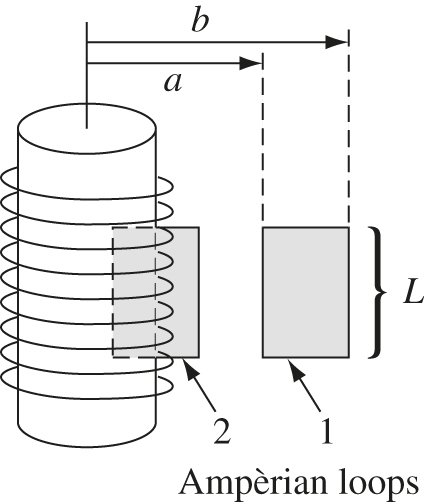
\includegraphics[width=0.25\textwidth]{figures/5_36.jpg}
\caption{\label{fig:1} A long solenoid has a constant $\mathbf{B}$-field inside, but no $\mathbf{B}$-field outside.}
\end{figure}

\vspace{3cm}

\section{Amp\`{e}re's Law}

\begin{enumerate}
\item (a) Show that if $\nabla \cdot \mathbf{B} = 0$, then we may write $\mathbf{B}$ as the curl of another vector, $\mathbf{A}$.  (b) Using Amp\`{e}re's Law, show that
\begin{equation}
\nabla \times \nabla \times \mathbf{A} = \nabla\left(\nabla \cdot \mathbf{A}\right) - \nabla^2 \mathbf{A} = \mu_0 \mathbf{J}
\end{equation}
(c) If we set $\nabla \cdot \mathbf{A} = 0$, then show that $\nabla^2 \mathbf{A} = -\mu_0 \mathbf{J}$. \\ \vspace{4cm}
\item Let the \textit{magnetic flux}, $\Phi_{\rm B}$ be defined like
\begin{equation}
\Phi_{\rm B} = \int \mathbf{B} \cdot d\mathbf{a}
\end{equation}
Show that
\begin{equation}
\Phi_{\rm B} = \oint \mathbf{A} \cdot d\mathbf{l}
\end{equation} \\ \vspace{2cm}
\item Apply the previous result to the long solenoid in Fig. \ref{fig:1}.  Orient the inner $\mathbf{B}$-field along the z-axis.  (a) What is the magnetic vector potential inside the solenoid?  (b) Outside the solenoid? (c) Use the cylindrical curl to obtain the $\mathbf{B}$-field from the vector potential.\footnote{Note that the vector potential is not zero outside the solenoid.} \\ \vspace{4cm}
\end{enumerate}

\end{document}
